\singlechapter{Skill Levels \label{chap:skill}}

\section{Purpose of the Skill Levels}
These achievement skill levels have been complied from years of research and surveys among unicyclist from all over the world.
They are intended to encourage unicyclists to progress at an even pace over a wide variety of unicycling skills.
These levels are not connected to the competition rules, other than in descriptions of how the skills are to be performed.
Skill levels are useful for helping riders determine a sequence of skills to learn, and to give them ideas for things to try.

\section{Testing of the Skill Levels}

\subsection{Official IUF Skill Level Testers}
The IUF Executive Board authorizes official level testers every two years at Unicon, the International Unicycling Championships and Convention, and at miscellaneous times throughout the year at Regional Clinics.
Any member of the IUF has the potential of being an official tester through the annual IUF Official Skill Level Clinic or Regional Clinic, both administered by a representative appointed by the IUF executive board.
Any member of the International Unicycling Federation may test Level 1 through 3 without going through certification.

\subsection{Becoming an Official Tester}
To become an official skill level tester, an IUF member needs to:
\begin{itemize}
\item Attend the Biannual Skill Level Clinic, offered three to five times during Unicon every two years, or attend a regional clinic, offered by miscellaneous officials throughout the year.
\item Fill out the Skill Level Tester Confirmation Form, available at the clinics.
\item Agree to follow all rules and guidelines presented in the clinic.
\end{itemize}


\subsection{IUF Biannual Skill Level Clinic and Regional Clinics}
The IUF Biannual Skill Level Clinic is a thorough explanation and demonstration of the 10 Official Skill Levels and corresponding rules for potential IUF Official Skill Level Testers.
This clinic will assist in creating a uniform standard of level testing throughout the world.
The Regional Clinics contain the same information and certification program as the Biannual Clinics but are taught at various times throughout the year, to be published on the IUF website.

The purpose for future IUF Skill Level Testers to attend the Biannual Skill Level Clinic or Regional Clinic is to:
\begin{itemize}
\item Qualify to become an Official IUF Skill Level Tester.
\item Be able to recognize and understand all skills in the skill levels.
\item Be able to test at a very accurate, consistent, and professional level.
\item View demonstrations of all skills in levels 1 through 10.
\item Have unanswered questions presented, discussed, and resolved.
\item Be able to understand all rules stated on the skill level card as well as in the IUF Official Rulebook, part \ref{part:skill}.
\end{itemize}
Other Clinic Information:
\begin{itemize}
\item Length of each Level Clinic will vary, with an approximate time allotment of one hour.
\item Leader of each clinic will be available following each clinic to answer any unanswered questions.
\end{itemize}

\subsection{Skill Level Tester Confirmation Form}
In addition to attending the Biannual Skill Level Clinic or Regional Clinic, potential testers are also required to sign the Skill Level Tester Confirmation Form, which are available upon completion of the clinic and tutorial.
By signing this document, the potential tester agrees to all rules and responsibilities presented in part \ref{part:skill} of the IUF Rulebook.
Signing also confirms their decision to become certified as an IUF Official Level Tester.
Each potential tester will also be asked to state the level he/she desires to be able to test to.
All completed forms will be examined and considered by the IUF Skill Level Director and within 30 days of signing, an email certification will be sent to all potential testers.
From the day the certification is sent, potential testers have up to 15 days to appeal to the IUF Executive Board for a re-evaluation (for example more levels desired to test than actually granted).

\subsection{Responsibilities of an Official Skill Level Tester}
Once an IUF member is confirmed as an Official Skill Level Tester, he/she is required to:
\begin{itemize}
\item Submit all passed skill levels to the IUF by sending them to the current International Skill Level Director's email address.
Submit the name of the person tested, the level(s) passed, the date each level was passed, and the name(s) and country number(s) of the level tester (if applicable).
All levels passed by members are stored in the IUF database.
The level tester must be certified to test the level of the submitted passed skill level.
For Level 8 and above, two certified testers for Level 8 and above must be submitted for verification.
Exceptions may be made by the IUF executive Board on a case-by-case basis, prior to testing.
\item Attend the Biannual Skill Level Clinic and/or Regional Clinic every other year for testing renewal.
This allows for each tester to refresh his/her knowledge as well as get updated on newly passed guidelines.
Certified skill level testers may also be granted permission to teach mini skill level clinics within their country's national convention, clubs or others not within a club, as determined by the IUF.
\item Follow completely and accurately all rules and guidelines presented in part \ref{part:skill} of the IUF Rulebook.
Any questions or concerns must be directed towards the International Skill Level Director immediately.
Failure to do so will result in restrictions and/or loss of ability to test.
\item The IUF will provide testers with a standard template for certificates that can be printed out and given to riders upon completion of each level.
\end{itemize}

\subsection{Restrictions for Official Level Testers}
Questionable knowledge will be confirmed by the International Skill Level Director through personal discussions, practice test situations, and/or outside connections to the potential tester prior to level testing confirmation.
\begin{itemize}
\item Testers are unable to test their own family members.
\item Testers must be at least 14 years old to qualify.
\item Riders and non-riders can test to the level in which he/she has the greatest proven knowledge (as decided by the International Skill Level Director).
\end{itemize}

\subsection{Recognition of Skill Levels}
All Skill Levels successfully passed are to be submitted to the IUF Skill Level Director every six months.
Once submitted, the IUF Skill Level Director will verify the levels.
Any Official Skill Level Tester from any country may test levels, as long as the guidelines highlighted in the IUF Rulebook, part \ref{part:skill}, are accurately followed.
National organizations must recognize all verified Skill Levels by the IUF independent of the country in which specific levels.

\section{Guidelines of the Skill Levels}

\subsection{General}
\begin{itemize}
\item Rider must perform all skills in the level at the first attempt except for three skills maximum, which must be performed at the second attempt.
This means only one mistake for each skill and maximum of three mistakes per
level.
\item All preceding levels must be passed prior to testing for a higher skill level.
\item All skills (except mounts) must begin and end with the rider sitting on the seat, feet on the pedals, and riding in control for at least three revolutions before and after each skill (complete cycles of the wheel).
\item Skills in each level can be performed in any order.
\item Rider cannot use any external aids during any part of the test for any level.
These include walls, other people, etc.
\item Within a specific level test, the rider must use the same unicycle to pass all skills within that level.
\item All skills within a level must be performed within one hour of the beginning of the test.
\item During the test, the rider may not practice any skills for that level.
(They should not be allowed on their unicycle unless they are certainly testing!)
\item Riders may only test once per day.
Exceptions will be given by consent of the IUF's Executive Board.
\item Interference (for example another rider obstructing the rider's path) to a testing rider is up to the discretion of the tester(s).
If the tester rules interference, the rider has another opportunity to complete the interfered skill.
Interference will be based upon visual evidence, outside witnesses, and the integrity of the rider.
\end{itemize}

\subsection{Levels 8 and Above}
\begin{itemize}
\item Two official testers are required for Levels 8, 9, and 10.
It is recommended to have two testers for all levels past Level 5.
\item When testing levels 8 and above, it is highly recommended that the rider perform up to three easier skills before testing more difficult skills in the level.
For example, if a rider is struggling with hand wheel walk, he/she may choose to do three consistent skills before having to attempt hand wheel walk.
This allows for the rider to ease into the testing, but also allows the tester to be relieved of any significant time burdens.
\end{itemize}

\subsection{Circles and Figure Eights}
All circle figures must be greater than 1 meter and less than 8 meters in diameter.
The same applies for each half of the figure eights, between 1 and 8 meters for each circle (unless stated otherwise, as in Levels 2 and 3).

\subsection{Foot Placement for One-Foot Skills}
For all riding (forward and backward) and idling one-foot skills (Levels 4-10), the non-driving foot can be put anywhere the rider desires as long as it is completely out of contact with the pedal and wheel.

\subsection{Seat Out Skills}
In seat out figures, the seat may touch the rider's body but no weight may rest upon it (example: a rider may not sit on the front handle of a saddle during seat in back).
The seat may be held, taken out, and returned back to sitting with 1 or
2 hands.
However, for seat in front one-foot in Level 9, the seat may \textbf){not} come in contact with any part of the body.

\subsection{Hopping and Hop-Twist Skills}
For any hopping or hop-twist skills, the seat may be held with one, two, or no hands.

\subsection{Idling Skills}
One idle is a complete back and forth motion of the wheel.

\section{Descriptions of Specific Skills}
For any skill description and clarification not listed here, refer to the IUF Standard Skill rules (in chapter \ref{chap:freestyle_std-skill-rules}) and the Standard Skills List (chapter \ref{chap:freestyle_std-skills-list}).
To pass levels, all skills must be performed as described.

\subsection{Level 1: Ride 50 meters}
In Level 1, the rider must ride 50 meters (36 revolutions on a typical 20$"$ unicycle).
Do not just assume that the length around the gym is 50 meters.

\subsection{Level 2/3/4: Sharp 90/180/360 Degree Turns}
Turns must be made within a 1 x 1 meter square.
Rider must be riding in a straight line prior to entering the square (for example no riding in a spiral and finally doing a 360 degree turn at the end of the spiral) and must be riding in a straight line after coming out of the square.
Riding must be done as diagrammed below.
Riders may turn in excess of the angle required, but not less.

\begin{figure}[h]
\begin{center}
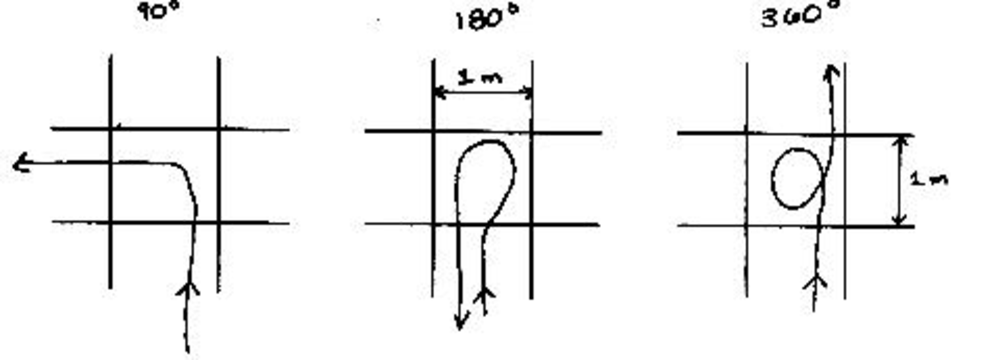
\includegraphics{degree_turns}
\end{center}
\vspace{-20pt}
\vspace{-10pt}
\end{figure}
 
\subsection{Level 3: 10 x 10 cm Obstacle}
The obstacle should be a rigid solid object.
The rider can ride or jump (forward or sideways) over the obstacle, using no external aids, as long as rider begins and ends the skill on the unicycle.

\subsection{Level 3: Hop 5 Times}
No external aids (bungee cords, toe clips, etc.), may be used for hopping.
The rider cannot travel more than 1 meter sideways while performing the skill.
The rider cannot rotate more than 180 degrees during the skill.

\subsection{Level 4/5: Idle 25 Times}
A rider cannot travel more than 1 meter sideways during the skill.
The rider cannot rotate more than 180 degrees during the skill.

\subsection{Level 5: Hop-Twist 90 Degrees}
Rider can be hopping prior to the execution of the skill.
90 degree Hop-twist must be a minimum of 90 degrees and a maximum of 135 degrees.

\subsection{Level 5/6: Seat on Side}
Seat and/or arm and hand can touch the body during this skill.
Seat on side to the right and left may be performed with the seat remaining on the same side for both.

\subsection{Level 6: Backspin/Frontspin}
An adequate backspin/frontspin is a continuous, linear motion by the body while the wheel changes direction.
The motion should be fluid, not like a turn, stop and turn.
The proper path looks like a cusp.
The change of direction must be performed within $\frac{1}{2}$ a wheel-revolution.
This illustration is a backspin.
For a frontspin reverse the riding direction.

\begin{figure}[h]
\begin{center}
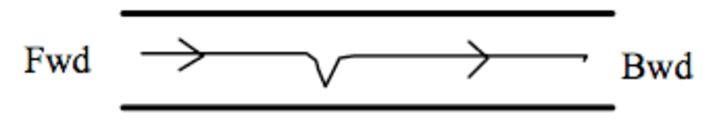
\includegraphics{fwd_bwd}
\end{center}
\vspace{-20pt}
\vspace{-10pt}
\end{figure}

\subsection{Level 6/7/8: Spins}
Spins must be performed within a 1 meter circle around a fixed point---no wandering spins.
Rider must perform 5 full rotations, but may need more than 5 full pedal rotations to complete these five spin rotations; no pirouettes are allowed.

\subsection{Level 7/8/9/10: Wheel Walk One-Footed}
This skill must be executed the full distance with the same foot always in control.
This skill may be performed with the non-pushing foot on the frame or extended.
A rider may not glide more than 1/2 revolution of the wheel during walk the wheel one-footed skills.

\subsection{Level 7: 180 Degree Hop-Twists}
Rider may be hopping prior to the execution of the skill.
180-degree hop-twist must be a minimum of 180 degrees and a maximum of 225 degrees.

\subsection{Level 8: Glide for 10 meters}
Gliding must be done on a level surface (not a slope).
The rider may not push the wheel during a glide (except for before and after the 10 meters of gliding for transitions).
During a glide there must be no contact with the pedals (except for before and after the 10 meters of gliding for transitions).
Gliding may be performed with the second foot on or off the frame.
During gliding, the rider is not allowed to coast (except for before and after the 10 meters of gliding for transitions).

\subsection{Level 8: Hand Wheel Walk}
Rider may be sitting on the seat \textbf{or} with the stomach on the seat.
However, the rider's feet may not touch the wheel, pedals, or the ground.

\subsection{Level 8/9: Pirouettes}
Pirouettes are three full 360-degree rotations and they must be performed with rider and unicycle rotating on a vertical axis.
There should be no pedal movement (forwards or backwards) during the pirouette.
When testing for pirouettes in Level 8 and 9, two testers must watch the pirouettes and come to a mutual agreement.
A rider must ride at least one revolution forwards before performing the forward pirouette.
A rider must ride at least one revolution backwards before performing the backwards pirouette.

\subsection{Level 9: Drag Seat in Front/Back}
When picking up drag seat in front/back, a rider may use either his/her hands or feet.

\subsection{Level 9: Seat in Front One-Footed for 10 Meters}
The rider shall have no contact with the seat other than the hand or hands holding the seat.
The hand(s) holding the seat as well as the corresponding arm(s) shall be extended away from the rider's body and shall not touch any part of the rider's body.

\subsection{Level 10: 180 Unispin}
The unicycle or the body of the rider must turn 180 degrees in a 180-unispin.
This skill may begin with hopping (seat out in front, or otherwise).
The rider must land the jump with both feet on pedals and the skill may end with the seat in
front or sitting on the seat.

\subsection{Level 10: Sideways Wheel Walk for 10 Meters}
Sideways wheel walk may be done with one or both feet.
Rider may not glide more than half revolution during the skill.

\subsection{Level 10: Coasting for 10 Meters}
During coasting you are not allowed to glide (except for before and after the 10 meters of coasting for transitions).
During coasting the rider may not come in contact with the wheel or pedals (except for before and after the 10 meters of coasting for transitions).
Must be performed on a level surface.
Coasting may be performed with either or both foot on the frame or extended.

\subsection{Level 10: Side Ride for 10 meters}
During side ride the rider may touch the seat with hands and body.
The rider's body from the waist down must be on one side of the unicycle.
The rider may choose how to hold the seat with either hands or forearms.
The controlling foot must be on the non-corresponding pedal (for example left foot on right pedal) and the other leg may not touch the unicycle.

\section{Mount Guidelines of the Skill Levels}

\subsection{General}
\begin{itemize}
\item For Level 3 and above, riders may not count their left and right foot mounts as different mounts.
\item The rider must declare his or her mount before being able to perform to the tester.
\item If a rider falls during the first attempt of the mount and/or ending, the rider must use that mount (and ending) for the second attempt.
\item The rider \textbf{must} end the mount by sitting on the seat with both feet on the pedals and riding a minimum of 3 revolutions.
For mounts that end in skills besides riding, the rider must do at least three revolutions, idles, or hops in the mounted position, and then end by sitting on the seat with both feet on the pedals and riding a minimum of three revolutions.
\item For Level 3 and above, riders must use the mounts clearly defined in section \ref{subsec:skill_mount-guidlines_mounts-for-level-3-and-above} of the IUF Rulebook.
No other mounts will be permitted by the IUF for reason of accurate and consistent level testing.
In addition, a rider may use a more difficult mount than the level he/she is testing for (for ekample mount to hop on wheel may be used for Level 4).
\item For Level 7 and above, riders must mount to a skill defined in section \ref{subsec:skill_mount-guidlines_mounts-for-level-3-and-above} of the IUF Rulebook.
No other mountsor skills will be accepted.
\end{itemize}


\subsection{Mounts for Level 3 and above \label{subsec:skill_mount-guidlines_mounts-for-level-3-and-above}}
A testing rider is required to choose his/her mounts for Level 3 and above from the list below.
No other mount variations will be accepted by the IUF.
All selected mounts may be used once per test, but for Level 7 and above the ending skill may be repeated (skills such as wheel walk, 1 foot, seat in front, etc.).
Definitions for these mounts can be found in the Standard Skill portion, section \ref{chap:freestyle_std-skills-list}, of the IUF Rulebook.

\begin{multicols}{2}
\textbf{Level 3}
\begin{itemize}
\item Standard mount
\item Back mount
\item Rolling mount
\item Side mount
\item Reverse side mount
\item Jump mount
\end{itemize}

\textbf{Level 4}

Same as above, plus:
\begin{itemize}
\item Side jump mount
\item Spin mount 180 degrees
\item Floor mount
\end{itemize}
\columnbreak

\textbf{Level 5}

Same as above, plus:
\begin{itemize}
\item Kick up mount
\item Swing up mount to seat in front [Standard Skill 312a]
\end{itemize}

\textbf{Level 6}

Same as above, plus:
\begin{itemize}
\item Mount to wheel walk
\item Mount to hop on wheel
\end{itemize}
\end{multicols}

\textbf{Level 7 through 10}

All mounts must end in a skill as defined below:
\begin{multicols}{2}
\begin{itemize}
\item Standard mount to one foot / seat in front
\item Back mount to wheel walk / one foot idling
\item Side mount to seat on side / wheel walk
\item Rolling mount to one foot / gliding
\item Jump mount to seat in front / wheel walk
\item Floor mount to wheel walk / stand up wheel walk
\item Kick up mount to wheel walk
\item Swing up mount to seat in front [Standard Skill 312a]
\item Mount to hop on wheel
\item Mount to stand up wheel walk
\item Mount to drag seat in front
\item Mount to hand wheel walk
\item Mount to side hopping
\item Side jump mount to wheel walk / seat in back / 1ft idling
\item Mount to sideways wheel walk
\item Mount to side ride
\item Spin mount 360 degrees
\item Seat in front pick up mount [Standard Skill 311a]
\item Mount to seat in side stand-up wheel walk
\item Mount to crank idle
\end{itemize}
\end{multicols}

\newpage
\begingroup
 \small
\begin{multicols}{2}
\textbf{LEVEL 1}\\
mount unicycle unassisted\\
ride 50 meters\\
dismount gracefully with unicycle in front\\\\
\textbf{LEVEL 2}\\
mount with left foot\\
mount with right foot\\
ride 10 meters between two parallel lines 30 cm apart\\
ride a figure eight with circle diameters smaller than 3 meters\\
ride down a 15 cm vertical drop\\
make a 90 degree turn to the left inside a 1 meter square\\
make a 90 degree turn to the right inside a 1 meter square\\\\
\textbf{LEVEL 3}\\
demonstrate 3 types of mounts\\
ride a figure eight with circle diameters smaller than 1.5 meters\\
come to a stop, pedal half a revolution backward and continue forward\\
ride with the stomach on the seat for 10 meters\\
make a 180 degree turn to the left within a 1 meter square\\
make a 180 degree turn to the right within a 1 meter square\\
hop 5 times\\
ride or hop over a 10 x 10 cm.
obstacle\\\\
\textbf{LEVEL 4}\\
demonstrate 4 types of mounts\\
ride backward for 10 meters\\
ride one footed for 10 meters\\
idle with left foot down 25 times\\
idle with right foot down 25 times\\
ride with seat out in front (against body) for 10 meters\\
ride with the seat out in back (against body) for 10 meters\\
make a 360 degree turn to the left inside a 1 meter square\\
make a 360 degree turn to the right inside a 1 meter square\\
\columnbreak

\textbf{LEVEL 5}\\
demonstrate 5 types of mounts ride backward in a circle\\
ride one footed in a figure eight\\
idle one footed with the left foot 25 times\\
idle one footed with the right foot 25 times\\
ride with seat out in front (against body) in a circle\\
ride with the seat out in back (against body) in a circle\\
ride with the seat on the side (against body) in a circle\\
hop-twist 90 degrees to the left\\
hop-twist 90 degrees to the right\\
walk the wheel for 10 meters \\
\\
\textbf{LEVEL 6}\\
demonstrate 6 types of mounts\\
ride backward in a figure eight\\
ride with the seat out in front (against body) in a figure eight\\
ride with the seat out in back (against body) in a figure eight\\
ride backward with the seat out in front (against body) for 10 meters\\
hop standing on wheel 5 times\\
ride with the seat on the side (against body) in a circle to the left\\
ride with the seat on the side (against body) in a circle to the right\\
ride one footed with the left foot for 10 meters\\
ride one footed with the right foot for 10 meters\\
back turn\\
front turn\\
spin \\
\newpage
\textbf{LEVEL 7}\\
demonstrate 7 types of mounts\\
ride backward with the seat out in front (against body) in a circle\\
ride one footed with the left foot in a circle\\
ride one footed with the right foot in a circle\\
walk the wheel in a circle\\
walk the wheel one footed for 10 meters\\
hop-twist 180 degrees to the left\\
hop-twist 180 degrees to the right\\
ride backward with the seat out in back (against body) for 10 meters\\
spin to the left\\
spin to the right\\\\
\textbf{LEVEL 8}\\
demonstrate 8 types of mounts\\
ride one footed with the left foot in a figure eight\\
ride one footed with the right foot in a figure eight\\
walk the wheel in a figure eight\\
walk the wheel one footed in a circle\\
ride backward one footed for 10 meters\\
glide for 10 meters\\
hand wheel walk for 10 meters\\
pirouette\\
backward spin\\
\columnbreak

\textbf{LEVEL 9}\\
demonstrate 9 types of mounts\\
walk the wheel one footed in a figure eight\\
ride backward one footed in a circle\\
ride backward with the seat out in front (against body) in a figure eight\\
ride backward with the seat out in back (against body) in a circle\\
walk the wheel one footed with the left foot for 10 meters\\
walk the wheel one footed with the right foot for 10 meters\\
walk the wheel backward for 10 meters\\
drag seat in front for 10 meters\\
drag seat in back for 10 meters\\
ride backward one footed with the left foot for 10 meters\\
ride backward one footed with the right foot for 10 meters\\
one footed with the seat out in front for 10 meters\\
backward pirouette\\\\
\textbf{LEVEL 10}\\
demonstrate 10 types of mounts\\
ride backward with the seat out in back (against body) in a figure eight\\
ride backward one footed in a figure eight\\
walk the wheel one footed with the left foot in a circle\\
walk the wheel one footed with the right foot in a circle\\
walk the wheel backward in a circle\\
180 uni spin\\
sideways wheel walk for 10 meters\\
coast for 10 meters\\
side ride for 10 meters\\
walk the wheel one footed backward for 10 meters\\
\end{multicols}
\endgroup